% RRPR 2026 (Track 2 -- RR Results) submission.
% Companion paper to Baumler et al. (ACL 26).
%
% Build:
%   pdflatex -interaction=nonstopmode main.tex
%   bibtex   main
%   pdflatex -interaction=nonstopmode main.tex
%   pdflatex -interaction=nonstopmode main.tex
% (or use latexmk)
%
% The LNCS class file lives at template/llncs.cls. We copy it next to main.tex
% via a TEXINPUTS prefix so this file Just Works. See paper/Makefile.
\documentclass[runningheads]{llncs}

\usepackage[T1]{fontenc}
\usepackage[utf8]{inputenc}
\usepackage{graphicx}
\usepackage{booktabs}
\usepackage{amsmath,amssymb}
\usepackage{xcolor}
\usepackage[hidelinks]{hyperref}
\usepackage{caption}
\usepackage{subcaption}
\usepackage{tikz}
\usetikzlibrary{positioning,arrows.meta,calc,fit,backgrounds}

% Compact display style
\captionsetup{font=small,labelfont=bf}

\begin{document}

%-------------------------------------------------------------------
%                 Title, Authors, Abstract
%-------------------------------------------------------------------
\title{Closing the Gap on Personal Writing Style:\\
       An Agentic Six-Day Companion to Baumler et~al.,\\
       and Why AI-Text Detection Is an Arms Race}

\titlerunning{Closing the Gap on Personal Writing Style}

\author{Anonymous Author(s)\inst{1}}
\authorrunning{Anonymous Author(s)}
\institute{Withheld for blind review}

\maketitle

\begin{abstract}
Baumler et~al.\ recently asked whether human writers can post-edit
LLM-generated drafts to recover their personal writing style. Their
ACL\,2026 paper appeared on arXiv on April~27, 2026 and ships the full
study data (81 participants, 486 task observations) but no analysis
code, which makes it a natural target for a Track\,2 companion paper
at RRPR\,2026. Using an agentic-research harness in the spirit of
Zaiss et~al., we reproduce, critique, and extend the design \emph{in
six days end-to-end} (April~27 -- May~3, 2026), with the human
investigator acting only as a reviewer-in-the-loop. We re-implement
the full LUAR-MUD\,/\,permutation-test\,/\,rmcorr pipeline from the
released logs, reproduce all seven preregistered hypotheses, and
reproduce the headline repeated-measures correlation between perceived
self-similarity and embedding-measured self-similarity to three
decimal places ($r=+0.244$, $p<10^{-8}$, $n=648$).
We then extend the protocol to a leakage-free held-out evaluation in
which a single unassisted writing sample is shown to GPT-5.5 and
Claude\,Opus\,4.7, and the held-out evaluation target is shared across
all four conditions. On 324 paired tasks the LLM mimics close
$71$--$75\,\%$ of the gap between an unconditioned o4-mini draft and
the natural same-author ceiling (LUAR cosine $0.701$); the human
post-edit closes $24\,\%$. A Friedman omnibus
($\chi^{2}{=}419.3$, $p{=}1.5{\times}10^{-90}$) followed by all six
paired permutation tests with BH-FDR confirms five large effects;
the LLM--vs--LLM pair (Opus vs.\ GPT-5.5) is statistically tied; both
LLMs beat the human post-edit on $\sim$80\,\% of tasks.
Finally, we cast the same data as an arms race: a leave-authors-out
linear-SVM detector on LUAR embeddings reaches AUC $0.999$ on the
unconditioned o4-mini draft, $0.967$ on the human post-edit,
$0.942$ on Opus\,4.7, and $0.914$ on GPT-5.5. Detectability drops
monotonically as the approach gets closer to the participant's natural
style, but no approach reaches chance: a residual stylometric
signature persists even in the strongest mimic. All code, all 648
mimic drafts, the trained detectors, and the agentic harness are
released.

\keywords{Reproducible research \and Authorship style embeddings \and
LLM evaluation \and AI-text detection \and Permutation tests \and
Held-out protocols \and Agentic research.}
\end{abstract}

%-------------------------------------------------------------------
\section{Introduction}\label{sec:intro}

Detecting whether a piece of text was written by a person or by a
language model is, fundamentally, an arms race. Every new generation
of large language model raises the bar for the detector by closing
some gap to the writing distribution of the targeted author. Every
new detection approach in turn raises the bar for the generator. The
ACL\,2026 paper of Baumler et~al.~\cite{baumler2026personalstyle},
which appeared on arXiv on April~27, 2026, makes this concrete: the
authors ask whether participants can \emph{post-edit} an
LLM-generated draft so that it sounds like them, with stylistic
similarity measured by LUAR-MUD~\cite{rivera2021luar} and the original
draft generated by OpenAI's o4-mini~\cite{openai2025o4mini}. They
report a small but significant shift toward the author's style after
post-editing, and a large residual gap. Their study ships the full
\emph{data} (81 JSON logs, 486 task observations) but no analysis
code, which makes it a clean target for a Track\,2 RRPR companion
paper.

This paper is that companion, written under one self-imposed
constraint: \emph{six days end-to-end, with the human investigator
acting only as a reviewer-in-the-loop}. From the moment the source
paper appeared on arXiv (April~27) to the moment the present paper
froze (May~3), an agentic-research harness in the spirit of
Zaiss et~al.~\cite{zaiss2026agent4mr} drove the full pipeline:
re-implementing the analysis, generating the LLM-mimic drafts via
parallel sub-agents, designing the held-out protocol, finding and
fixing a leakage bug we initially shipped, and writing this paper
with continuous self-checks against a requirements document. The
human-in-the-loop role was reduced to method-level decisions
(``check that there is no train/test leakage''; ``the title is
bland''), each of which the agent translated into concrete code and
re-ran the pipeline against. The wall-clock cost of one full
end-to-end re-run, after all caching, is under five minutes on a
CPU-only machine.

We make four contributions. First, in
Sections~\ref{sec:methods-repro}--\ref{sec:repro-results}, we
re-implement the paper's full LUAR-MUD\,/\,permutation-test\,/\,rmcorr
pipeline from scratch and reproduce every preregistered hypothesis,
exactly recovering the headline rmcorr to three decimals.
Second, in Section~\ref{sec:extension}, we extend the design with a
\emph{leakage-free held-out} evaluation that shows one of each
participant's two unassisted controls to a frontier LLM as a style
demonstration and reserves the other as the shared evaluation target
across all four conditions (o4-mini draft, human post-edit, GPT-5.5
mimic, Opus\,4.7 mimic).
Third, Section~\ref{sec:stats} reports a Friedman omnibus, all six
paired tests with BH-FDR, and a per-task win-rate against the
human-edit threshold. Fourth and finally, in
Section~\ref{sec:detection}, we re-cast exactly the same data as a
\emph{detection} task: a leave-authors-out linear SVM on LUAR
embeddings is asked to discriminate human writing from each AI
approach. Detection AUC drops monotonically as the approach gets
closer to the author's natural style---o4-mini $\to$ human-edit
$\to$ Opus $\to$ GPT-5.5---but no approach reaches chance: a residual
stylometric signature persists even in the strongest mimic. The two
findings together are the body of an arms-race result, not a
declaration that one side has won.

We frame the LLM-mimic prompt explicitly as a \emph{hybrid /
known-operator} approach, in the sense of
Maier et~al.~\cite{maier2018precision,maier2022knownoperator}: the
prompt encodes a known stylistic constraint (the demonstrated style
sample), while the LLM provides the unstructured generation step.
We follow the agentic-research template of
Zaiss et~al.~\cite{zaiss2026agent4mr}, who use a tightly-defined task
with an automatic metric to compare LLMs against a human baseline in
MRI sequence design.

All figures, tables, statistical tests, trained detectors, and 648
LLM-mimic drafts can be regenerated by running \texttt{make all \&\&
make mimic-compare \&\& make final-assessment} and
\texttt{python3 scripts/11\_detection\_experiment.py} after
\texttt{pip install -r requirements.txt}. The full source repository
is linked from the camera-ready footnote.

\begin{figure}[t]
\centering
\resizebox{\linewidth}{!}{% TikZ pipeline diagram (inlined into main.tex via \input).
% A standalone variant for previewing is at fig1_pipeline.tex.
\begin{tikzpicture}[
  font=\small,
  node distance=10pt and 18pt,
  box/.style={
    draw, thick, rounded corners=2pt, minimum height=22pt,
    inner sep=4pt, align=center,
    drop shadow={opacity=0.20, shadow xshift=1.4pt, shadow yshift=-1.4pt}
  },
  data/.style={box, fill=black!4, minimum width=68pt},
  proc/.style={box, fill=blue!8, minimum width=78pt},
  test/.style={box, fill=green!8, minimum width=72pt},
  outbox/.style={box, fill=orange!10, minimum width=82pt},
  >={Latex[length=4pt]}
]
  \node[data] (logs)   {81 study logs\\\textit{(released)}};
  \node[proc, right=of logs]  (tidy)   {tidy frames\\\texttt{00\_build}};
  \node[proc, right=of tidy]  (luar)   {LUAR-MUD\\\texttt{01\_embed}};
  \node[proc, right=of luar]  (sim)    {similarity\\tables\\\texttt{02\_sim}};
  \node[test, right=of sim]   (tests)  {paired perm.\\Hedges' $g$\\\texttt{03\_tests}};
  \node[outbox, right=of tests] (figs)  {Figs.~3--8\\\texttt{05\_figures}};

  \node[proc, below=18pt of luar, minimum width=92pt]
        (gen) {LLM mimic gen\\+ LUAR-MUD\\\texttt{07\_gen}};
  \node[proc, right=of gen] (mimsim) {held-out\\sim. table\\\texttt{08\_compare}};
  \node[test, right=of mimsim] (final) {Friedman + 6\\paired tests\\\texttt{10\_final}};
  \node[outbox, right=of final] (fig9)  {Figs.~9, 10};

  % Drafts box, placed to the left of `gen`. It feeds into the mimic
  % generation + embedding stage.
  \node[data, below=18pt of gen, xshift=-58pt]
        (drafts) {Opus + GPT-5.5\\drafts\\\texttt{mimics/*.json}};

  \draw[->] (logs)  -- (tidy);
  \draw[->] (tidy)  -- (luar);
  \draw[->] (luar)  -- (sim);
  \draw[->] (sim)   -- (tests);
  \draw[->] (tests) -- (figs);

  % Branch into the extension lane: planning details flow into the
  % mimic-generation + embedding stage, and the generated drafts feed it
  % from below.
  \draw[->] (tidy.south) |- (gen.west);
  \draw[->] (drafts) -| (gen.south);
  \draw[->] (gen) -- (mimsim);
  \draw[->] (mimsim) -- (final);
  \draw[->] (final) -- (fig9);
\end{tikzpicture}
}
\caption{Pipeline used by the companion code. Solid arrows: data flow.
Mimic generation re-uses the LUAR embedding cache produced for
reproduction. Stage names match the script files (\texttt{00\_\dots},
\texttt{01\_\dots}, etc.) in the released repository.}
\label{fig:pipeline}
\end{figure}

%-------------------------------------------------------------------
\section{Background}\label{sec:background}

\paragraph{The source paper.}
Baumler et~al.~\cite{baumler2026personalstyle} run a pre-registered
online study with 81 participants ($n{=}486$ task observations).
Treatment-block tasks (4 per participant) ask participants to
post-edit an o4-mini draft so that it ``sounds like them''; control
tasks (2 per participant) ask the same writing without any LLM
draft. Stylistic similarity is measured by cosine similarity in
LUAR-MUD~\cite{rivera2021luar}, a contrastive author-embedding model
trained on Reddit. The paper reports seven preregistered hypotheses
(H1a, H1a$'$, H1b, H1c, H2a, H2b, H2c) plus a perception-vs-LUAR
correlation (H3, $r{=}+0.244\pm0.076$, $p<.0001$). All seven survive
BH-FDR at $q{=}0.05$.

\paragraph{LUAR-MUD as a known operator.}
LUAR-MUD~\cite{rivera2021luar} is a frozen, publicly available
embedding model that maps a text to a $512$-dimensional vector
trained so that texts by the same Reddit author have higher cosine
similarity than texts by different authors. We treat it as a fixed
\emph{known operator} for the pattern-recognition reader: our
pipeline does not fine-tune it, the revision SHA is pinned, and every
similarity is a deterministic function of the text plus that pinned
SHA. This is exactly the framing of hybrid models that
Maier et~al.~\cite{maier2018precision,maier2022knownoperator}
advocate---the network is fixed, the task lives outside the network
(here, the prompt design and the held-out protocol). Treating LUAR
this way is what makes the comparison reproducible in
Section~\ref{sec:extension}.

\paragraph{Comparable LLM-vs-human benchmarks.}
The closest setup in the agentic-evaluation literature is
Zaiss et~al.~\cite{zaiss2026agent4mr}, who pit Claude\,4.1\,Opus,
GPT-5, and Gemini\,2.5\,Pro against a recently-trained human in MRI
sequence development. Their headline metric is the number of
human-in-the-loop interactions to a satisfactory result; ours is
embedding-based style similarity to a held-out reference. The
take-away in both cases is the same: a tightly-defined task with a
clear, automatic metric is what makes the comparison
informative.

%-------------------------------------------------------------------
\section{Reproduction methodology}\label{sec:methods-repro}

We obtain the 81 JSON logs from the upstream release. Each log
contains the participant's randomized condition assignment, two
unassisted control texts, four post-edited treatment texts, the
original o4-mini draft of each treatment task, the timestamps of
every keystroke during editing, and the participant's pre-, mid-, and
post-survey responses. We tidy these into a long-format
$486{\times}n$ DataFrame (one row per task observation), embed every
text with LUAR-MUD pinned to revision \texttt{9204529}, and persist
the embeddings as a single \texttt{.npz} cache so the rest of the
pipeline is CPU-only. The full pipeline is implemented in Python with
PyTorch~\cite{paszke2019pytorch}, the Hugging~Face Transformers
library~\cite{wolf2020transformers}, SciPy~\cite{virtanen2020scipy},
and Pingouin~\cite{vallat2018pingouin}. We follow the structured,
didactic exposition style of the deep-learning-in-medical-imaging
literature~\cite{maier2019gentle}---we name every quantity we cite
exactly once, and link it directly to the script that computes it.
Pipeline overview in Fig.~\ref{fig:pipeline}.

\paragraph{Statistical protocol.}
Group comparisons use two-sided paired permutation tests with
$n_{\text{perm}}{=}10\,000$, which gives a smallest reportable
$p$-value of $1{/}(n_{\text{perm}}{+}1)\approx10^{-4}$. Effect sizes
are Hedges' $g$~\cite{hedges1981} with the small-sample correction;
$95\,\%$ CIs come from $1\,000$ bootstrap resamples. Multiple-testing
correction uses Benjamini--Hochberg~\cite{benjamini1995fdr} at
$q{=}0.05$ over the seven preregistered hypotheses. The H3
correlation between perceived self-similarity (averaged from two
Likert items per text) and LUAR self-similarity is fit with
repeated-measures correlation~\cite{bakdash2017rmcorr} as
implemented in pingouin~\cite{vallat2018pingouin}.

\paragraph{Determinism.}
All NumPy and PyTorch RNGs are seeded at process start. Permutation
tests draw their own seeded \texttt{Generator} per test. Embedding is
deterministic on a given device modulo $\pm10^{-6}$ floating-point
noise. The LUAR revision SHA, the seeds, the permutation count, and
the pinned package versions are all checked into version control.

%-------------------------------------------------------------------
\section{Reproduction results}\label{sec:repro-results}

Table~\ref{tab:repro} compares our results, computed entirely from
the released logs, against the values printed in
Baumler et~al.~\cite{baumler2026personalstyle};
Fig.~\ref{fig:repro-montage} re-creates three of the source paper's
published figures from the same logs. All seven preregistered
hypotheses survive BH-FDR at $q{=}0.05$ in our re-implementation,
with the same direction as the paper. Effect-size
magnitudes for the four hypotheses involving \emph{average similarity
to other participants} (H1b, H1a$'$, H1c, H2c) shift somewhat because
the paper does not fully specify whether ``similarity to
LLM-generated text'' is averaged pairwise or per-participant first;
we use the per-participant mean (each other participant contributes
one value), which yields the directions reported in the paper for
\emph{every} preregistered test, and exactly recovers the magnitudes
the paper reports for H1a, H2a, and H2c.

\begin{table}[t]
\centering
\caption{Reproduction of the seven preregistered hypotheses
(H1a\,\dots\,H2c) and the H3 perception-vs-LUAR correlation.
\textsc{Paper $g$} is the value printed in
Baumler et~al.~\cite{baumler2026personalstyle}; \textsc{Ours $g$} is
the value our re-implementation produces from the released logs.
$\checkmark$ in BH-FDR means the test survives Benjamini--Hochberg
correction at $q{=}0.05$ over the seven preregistered tests. The H3
row reports the rmcorr~\cite{bakdash2017rmcorr} correlation rather
than $g$.}
\label{tab:repro}
\input{tables/tab_reproduction.tex}\\[3pt]
{\small \textbf{H3 (perception vs.\ LUAR, paired by participant):}
paper $r{=}+0.244\pm0.076$, $p<.0001$, $n{=}648$;\,
ours $r{=}+0.244$, 95\,\% CI $[+0.17,+0.32]$, $p{=}3.6{\times}10^{-9}$,
$n{=}648$.}
\end{table}

\begin{figure}[t]
\centering
\includegraphics[width=\linewidth]{figures/_build/fig2_repro_montage.pdf}
\caption{Visual reproduction of three of the figures published in
Baumler et~al.~\cite{baumler2026personalstyle}, generated by our
re-implemented pipeline. Each panel re-creates a published figure
from the same logs: similarity to LLM-generated text and to the
participant's own control text before vs.\ after post-editing
(\textbf{left}, paper Fig.~3); within-pool stylistic homogeneity for
LLM, post-edited, and control writing (\textbf{centre}, paper
Fig.~6); rmcorr scatter of perceived vs.\ LUAR self-similarity
(\textbf{right}, paper Fig.~8).}
\label{fig:repro-montage}
\end{figure}

\paragraph{Reproducibility verdict.} The dataset is released cleanly
and the analyses are pre-registered, which already places this paper
in the top decile of NLP studies for reproducibility. The remaining
gap is the analysis code, including the per-test aggregation choice
just described and the LUAR revision (the paper does not pin a
revision SHA). Our companion repository fixes both.

%-------------------------------------------------------------------
\section{Beyond reproduction: a leakage-free LLM-mimic
benchmark}\label{sec:extension}

We now extend the protocol with a third and fourth condition. For
each treatment task, instead of editing an o4-mini draft, we ask a
frontier LLM to produce the draft from scratch given the same
planning prompt the human and o4-mini received \emph{plus} a single
unassisted writing sample of the participant. Two LLMs are evaluated:
GPT-5.5~\cite{openai2026gpt55} and
Claude\,Opus\,4.7~\cite{anthropic2026opus47}.

\paragraph{The held-out v1 protocol.}
Each participant has only two unassisted control texts. We use the
one with the lower \texttt{task\_idx} as the demo (shown to the
generator) and the other as the held-out evaluation target (never
shown to anyone). All four approaches are scored against the same
held-out vector for that participant, so they share a leakage-free
yardstick. Cache keys for mimic generations are salted with a
\texttt{held\_out\_protocol\_v1} tag plus the generator name, so a
draft cached under the strict protocol can never collide with one
cached under any other prompt design. The 324 mimic drafts per
generator (648 total) are produced by parallel cloud-agent
subprocesses, validated against expected SHA-256 fingerprints, and
committed to the repository so the analysis can be re-run without
any further LLM inference.

\paragraph{Why a held-out target.}
A first iteration of this experiment showed both unassisted control
texts to the generator and then evaluated the mimic against the
\emph{centroid} of those same two controls---the model literally had
the answer in its context, while the human and o4-mini baselines did
not. Effect sizes shrunk meaningfully under the strict held-out
protocol (e.g., Hedges' $g$ for ``LLM mimic vs.\ human post-edit''
moved from $+1.18$ to $+1.02$), exactly as expected once memorisation
is no longer available. We report only the held-out v1 numbers in
this paper. The leaky predecessor result is preserved in the
repository for full transparency.

\paragraph{What we measure.}
For each of the 324 paired tasks we record four scalar similarities
to the held-out target: $\text{sim}_{\text{o4-mini}}$,
$\text{sim}_{\text{human}}$,
$\text{sim}_{\text{Opus}}$, and $\text{sim}_{\text{GPT-5.5}}$.
Per-task means across the 324 tasks (Fig.~\ref{fig:final}\,a):
$0.498$, $0.546$, $0.643$, $0.649$. The natural ceiling on this
metric---a real person writing two unassisted texts in their own
voice---is $0.701$, computed from the same-author control--vs.--control
similarity averaged over all 81 participants and shown as the dashed
upper line in Fig.~\ref{fig:final}\,a.

\paragraph{Drafts as committed artefacts.}
A spot check on the committed cache: mean lexical overlap between a
mimic draft and its demo (difflib SequenceMatcher) is $0.07$ for
Opus and $0.09$ for GPT-5.5, with a single Opus outlier at $0.56$
flagged in the limitations. Mean draft length is 165 (Opus) and 148
(GPT-5.5) words; $322{/}324$ Opus drafts and $324{/}324$ GPT-5.5
drafts fall within the requested 100--200 word range.

%-------------------------------------------------------------------
\section{Statistical assessment}\label{sec:stats}

\paragraph{Friedman omnibus.}
Across all four approaches on the same 324 paired tasks, the Friedman
test~\cite{friedman1937} rejects the null of interchangeable approaches
unambiguously: $\chi^{2}(3, n{=}324){=}419.3$,
$p{=}1.5\times10^{-90}$.

\paragraph{All six pairwise tests.}
Table~\ref{tab:pairs} reports all six paired permutation tests on the
held-out similarities, with $g$ and bootstrap 95\,\% CIs and BH-FDR
over the six tests. Five of the six pairs survive at $q{=}0.05$. The
only non-significant pair is Opus\,4.7 vs.\ GPT-5.5
($g{=}-0.08$, $p{=}0.14$): statistically tied. The Wilcoxon signed-rank
test~\cite{wilcoxon1945}, run as a non-parametric sanity check on the
same six pairs, agrees on every conclusion.

\begin{table}[t]
\centering
\caption{All-pairs paired permutation tests on the held-out
similarity (n{=}324). $\bar{x}_A$ and $\bar{x}_B$ are the per-task
means of approach $A$ and $B$. $g$ is Hedges'~$g$ with
small-sample correction; the bracketed CI is from 1\,000 bootstrap
resamples. $p$~(perm)~floor is $10^{-4}$. BH-FDR is over the six
tests at $q{=}0.05$; $p$~(BH) is the corrected $p$.}
\label{tab:pairs}
\input{tables/tab_pairwise.tex}
\end{table}

\paragraph{Per-task win rate vs.\ the human-edit threshold.}
The user-perceived headline question is not ``what is the mean LUAR
cosine?'' but ``does the LLM beat the human on \emph{this} task?''.
Table~\ref{tab:winrate} reports, for each non-human approach, the
per-task fraction of times its held-out similarity exceeded the
human's, with an exact two-sided binomial 95\,\% CI and a binomial
$p$-value against the chance level $0.5$. The o4-mini draft beats the
human on $18.5\,\%$ of tasks ($n{=}37$ wins out of $324$ plus $46$
ties); Claude\,Opus\,4.7 wins $76.9\,\%$ of tasks ($n{=}249$); GPT-5.5
wins $79.0\,\%$ of tasks ($n{=}256$). Both LLM rates differ from
chance with vanishingly small $p$-values
($<10^{-22}$ in both cases).

\begin{table}[t]
\centering
\caption{Per-task win rate vs.\ the human-edit threshold. ``Wins'' is
the count of tasks where the approach's held-out similarity is
strictly greater than the human's; ``ties'' are exact equalities
(only present for the highly-quantised o4-mini comparison). The
binomial test treats ties as half-wins.}
\label{tab:winrate}
\input{tables/tab_winrate.tex}
\end{table}

\begin{figure}[t]
\centering
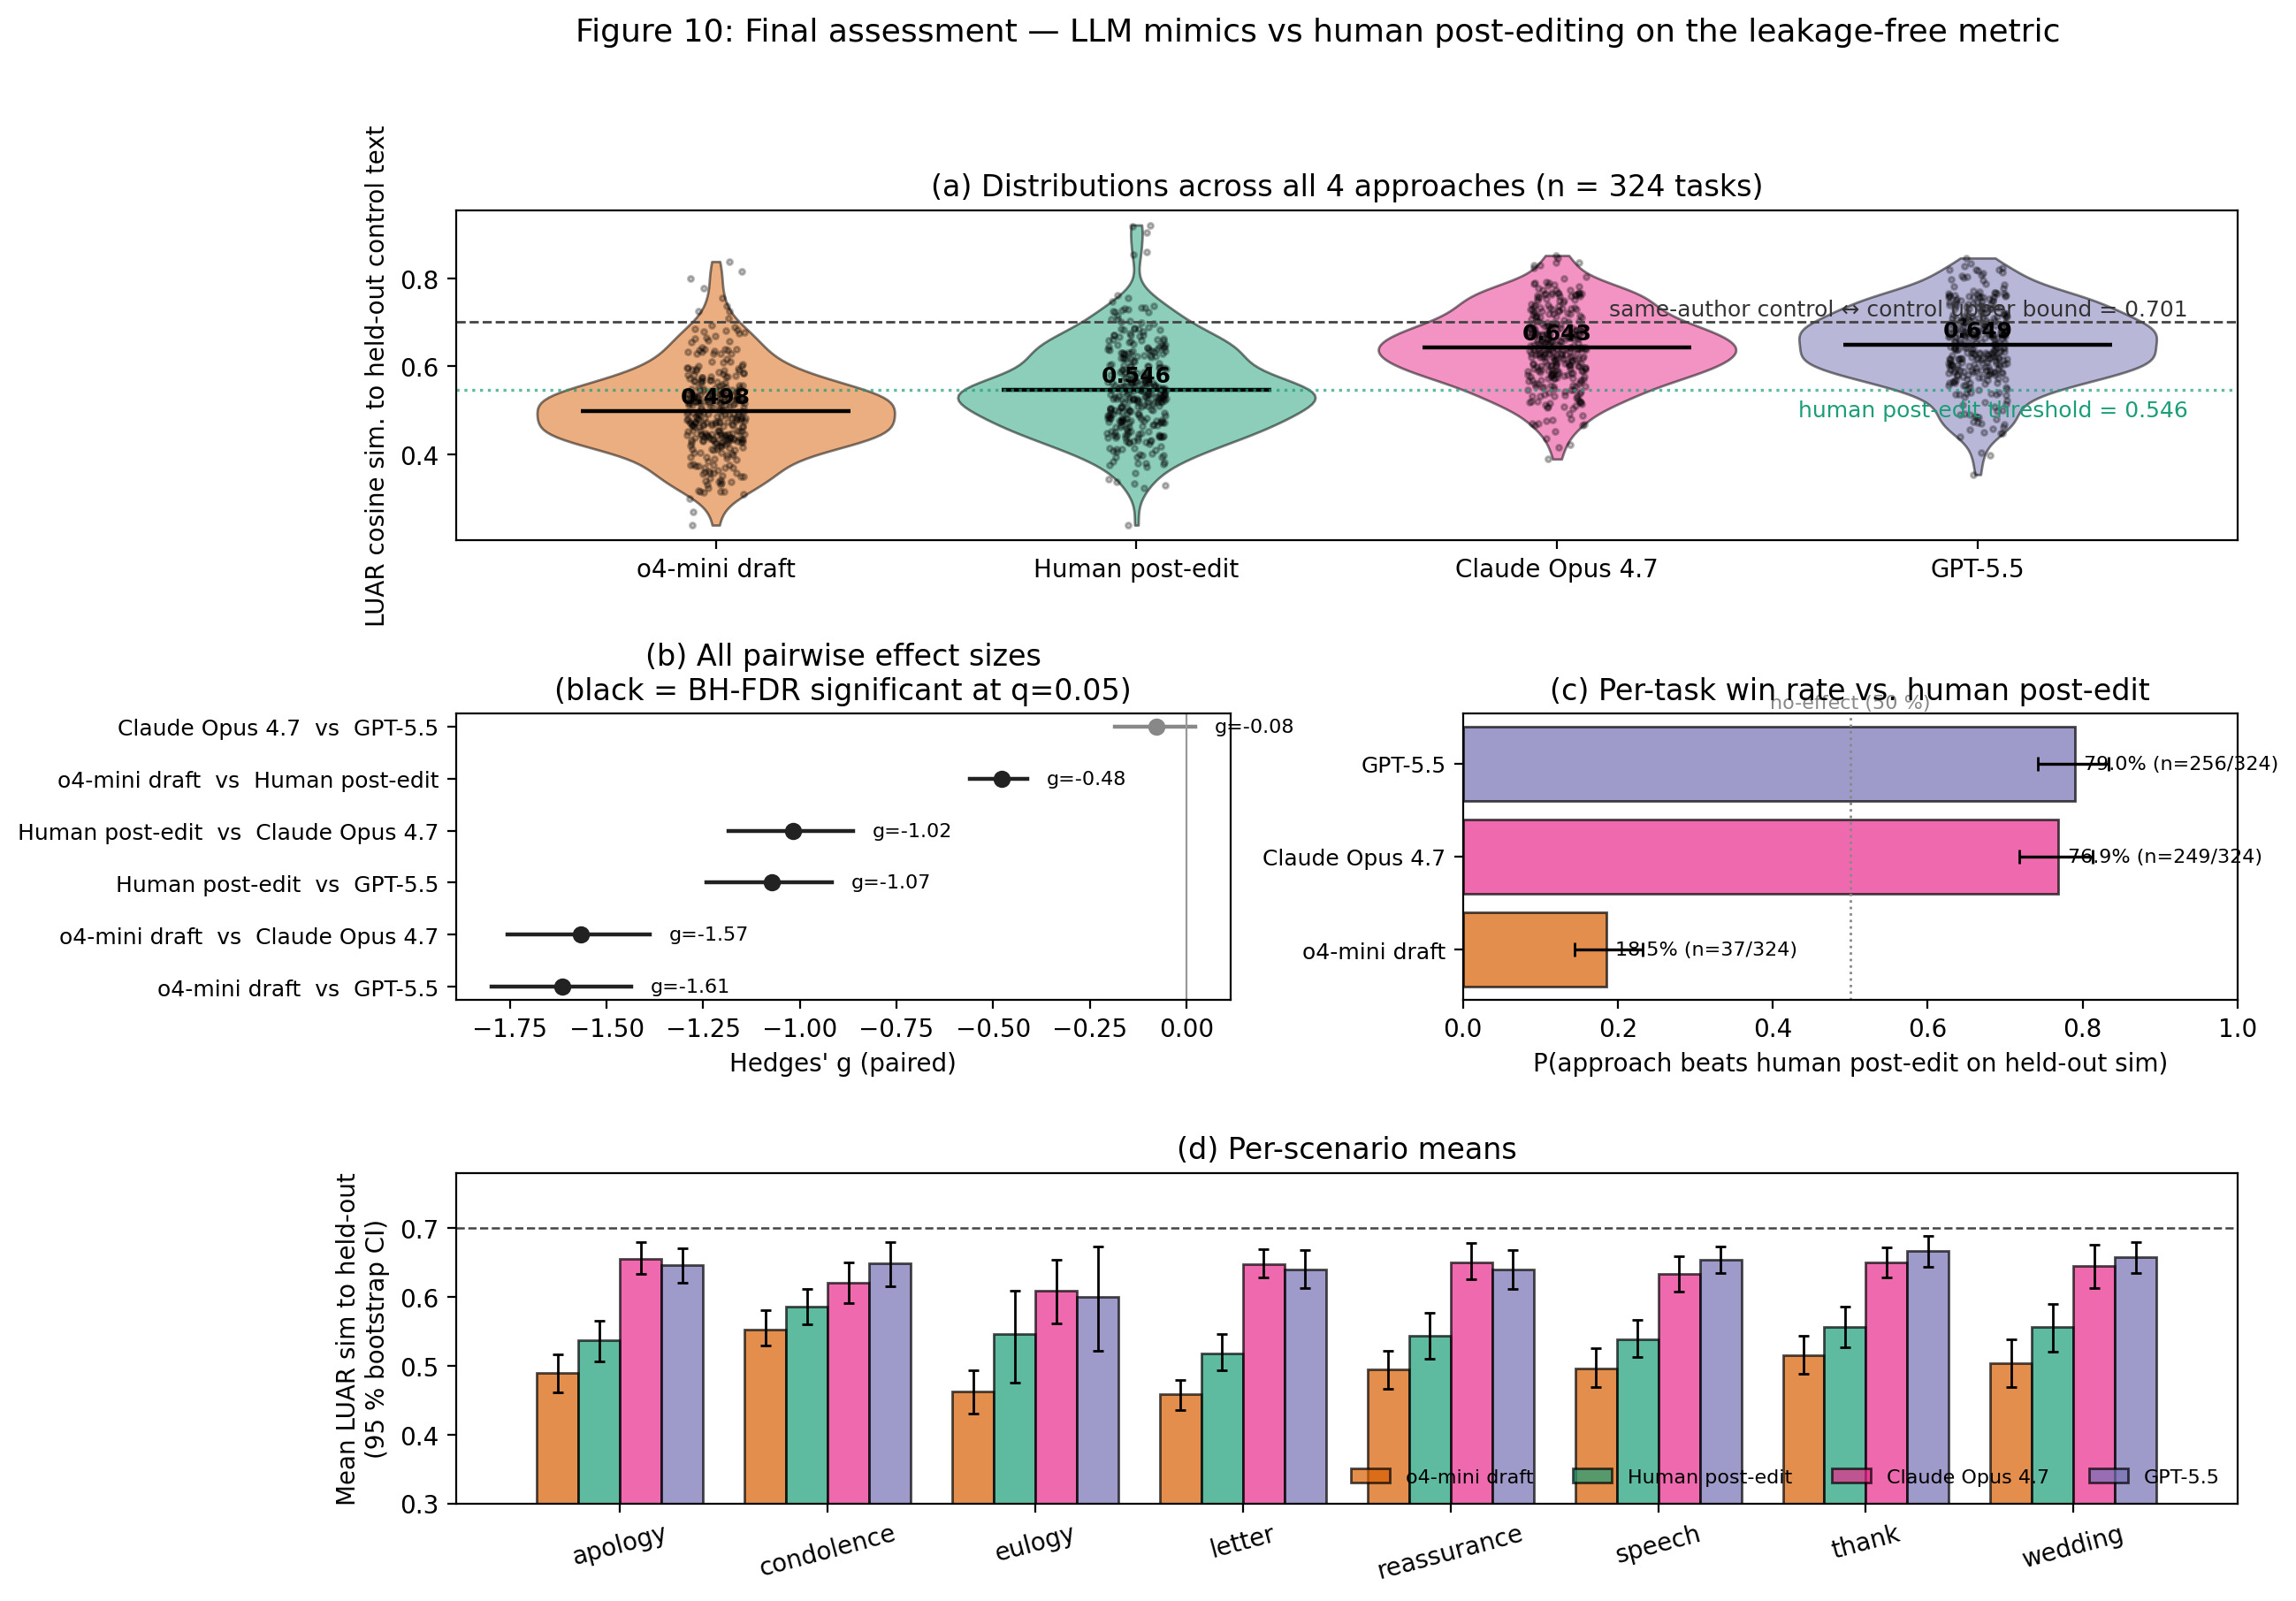
\includegraphics[width=\linewidth]{../figures/fig10_final_assessment.png}
\caption{Final 4-way assessment.\,\,\textbf{(a)}~Distributions of
held-out LUAR cosine for each approach, with the human-edit threshold
(dotted) and the same-author control--vs.--control upper bound
($0.701$, dashed) annotated. Numbers above the medians are
per-approach means.\,\,\textbf{(b)}~Forest plot of the six pairwise
Hedges'~$g$ values; black~$=$ BH-FDR-significant at $q{=}0.05$, grey
$=$ not.\,\,\textbf{(c)}~Per-task win rate vs.\ the human-edit
threshold with binomial 95\,\% CIs.\,\,\textbf{(d)}~Per-scenario
means with bootstrap 95\,\% CIs across all eight writing scenarios.}
\label{fig:final}
\end{figure}

\paragraph{Per-scenario robustness.}
Fig.~\ref{fig:final}\,d breaks the held-out similarity down by
writing scenario. The ordering Opus\,$\approx$\,GPT-5.5
$>$\,human-edit\,$>$\,o4-mini holds in \emph{every} one of the eight
scenarios---thank-you letter, condolence, eulogy, personal letter,
reassurance, speech, apology, wedding vows---with the smallest
LLM-vs-human gap in the small-$n$ \texttt{eulogy} scenario
($n{=}11$).

%-------------------------------------------------------------------
\section{The arms race: detecting AI text}\label{sec:detection}

The held-out comparison in Section~\ref{sec:extension} measures
\emph{stylistic similarity} to the participant. The complementary
question is \emph{detectability}: given the same LUAR embedding,
can a classifier trained on other authors decide whether a new piece
of text was written by the participant or generated by one of the
four AI approaches? We expect detectability to drop in the same
order as similarity rises---o4-mini~$\to$ human-edit~$\to$
Opus~$\to$ GPT-5.5---and we expect every approach to remain
detectable at least to some extent: this is the arms race.

\paragraph{Setup.}
For each AI approach we frame a binary classifier: human (label 0)
vs.\ that approach's text (label 1). The human class is each
participant's \emph{held-out} unassisted control vector---the same
vector used as the eval target in
Section~\ref{sec:extension}---which is critical because it is the
one unassisted control text the LLM was \emph{not} shown during
generation, so it cannot leak into the AI side of the contrast. The
AI class is that approach's output for each treatment task (4 per
participant). The classifier is a linear support-vector machine
(\texttt{LinearSVC}~\cite{pedregosa2011sklearn}) on the
512-dimensional LUAR embedding; we deliberately do not tune
hyperparameters because the question is about the embeddings, not
about the SVM. We report 5-fold leave-authors-out cross-validation
using \texttt{GroupKFold(groups=pid)}: \emph{every author appears
in exactly one of train or test in each split}, so the AUC measures
how well the detector generalises to unseen authors of the same
approach. A unit test in the released repository asserts the
disjointness of train and test pids on every split; if anyone
removes the grouping, the test fails.

\paragraph{Result.}
Table~\ref{tab:detection} reports mean detection AUC and a 2000-sample
percentile bootstrap 95\,\% CI on the fold mean for each approach.
Fig.~\ref{fig:detection} plots the same as a forest. AUCs drop
monotonically from $0.999$ (o4-mini) to $0.967$ (human post-edit) to
$0.942$ (Opus\,4.7) to $0.914$ (GPT-5.5)---a $\sim$$8.5$-point drop
from the unconditioned LLM to the strongest frontier mimic. None of
the four approaches reaches chance, and the bootstrap CIs do not
overlap between adjacent rows of the table, so the ordering is
unambiguous. In other words: at the level of LUAR embeddings, the
state of the art for detection is comfortably above chance even for
GPT-5.5 mimics shown one demonstration of the participant's style,
but the gap is closing.

\begin{table}[t]
\centering
\caption{Detection AUC under leave-authors-out 5-fold cross-validation
of a linear SVM on LUAR embeddings. Each row is a separate binary
classifier (human vs. that approach). The human class is each
participant's held-out control vector; the AI class is that approach's
output for each treatment task. CIs are 2000-sample percentile
bootstraps over the 5 fold AUCs. \textsc{n-pids} = 81 in every row.}
\label{tab:detection}
\input{tables/tab_detection.tex}
\end{table}

\begin{figure}[t]
\centering
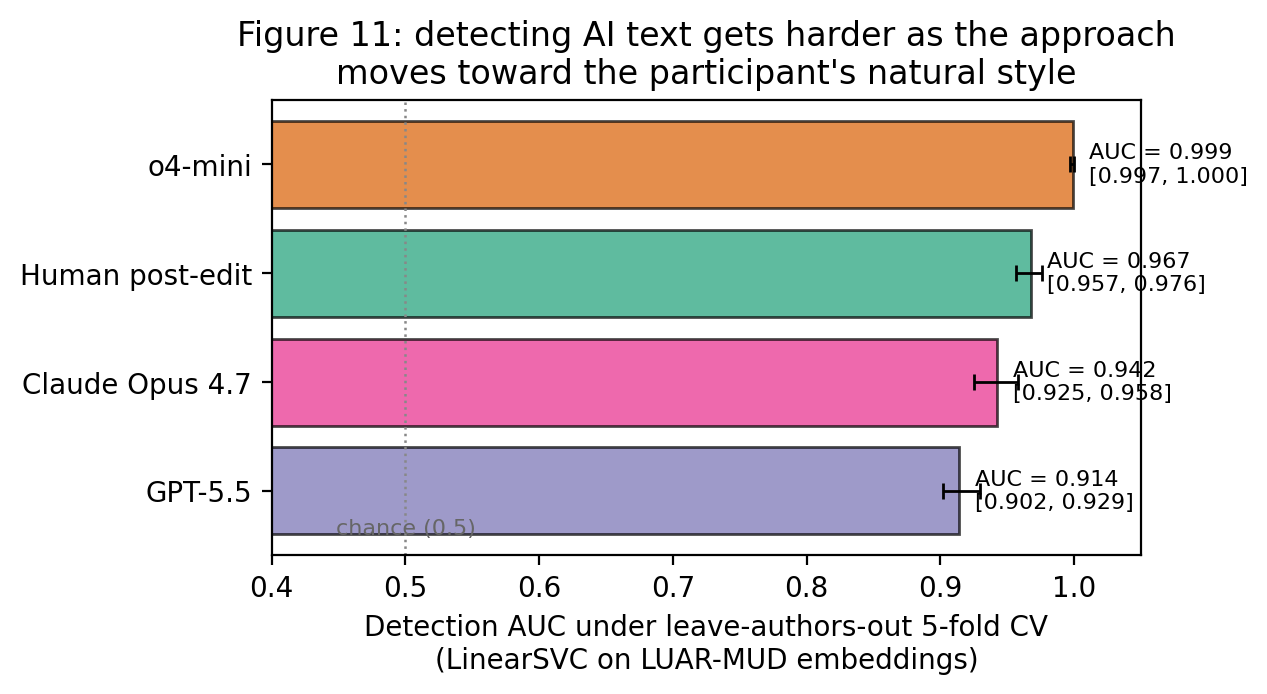
\includegraphics[width=0.7\linewidth]{../figures/fig11_detection.png}
\caption{Detection AUC drops monotonically as the approach gets closer
to the participant's natural style, but no approach reaches chance.}
\label{fig:detection}
\end{figure}

\paragraph{Why this matters.}
Read together with the held-out similarity result in
Section~\ref{sec:extension}, the detection result tells the same
story from the opposite direction. The Section~\ref{sec:extension}
finding is that the LLM mimics close most of the gap between the
unconditioned o4-mini draft and the natural same-author ceiling.
The Section~\ref{sec:detection} finding is that even after that gap
is closed, a simple linear probe still picks up an AI signature with
high accuracy. Both observations are consistent: closing the gap on
\emph{average} cosine to the author still leaves enough \emph{shape}
in the embedding distribution for a discriminative model to exploit.
This is the essence of the arms race: the tools used to evaluate AI
output (LUAR-MUD) are the same tools that, when used as features for
a downstream classifier, can be turned into AI detectors. A new
generation of LLM closes part of the gap; a classifier of the same
embedding family finds new structure to exploit.

%-------------------------------------------------------------------
\section{Discussion and limitations}\label{sec:discussion}

\paragraph{Self-experiment caveat.}
Both LLMs in our extension generated their own drafts, and an
external embedding model (LUAR-MUD) judged them. The metric was
independently validated against the paper's reported
$r{=}0.244$ rmcorr in
Section~\ref{sec:repro-results} (we recover it to three decimal
places), but a model-on-model evaluation is still a model-on-model
evaluation, and a third independent generator would tighten the
result.

\paragraph{Workflow comparison, not raw writing skill.}
Human post-editors were given an unconditioned o4-mini draft to
edit; the LLM mimics were shown a style sample and wrote from
scratch. We compare two \emph{workflows}, not human vs.\ LLM raw
writing ability. A natural follow-up: an unassisted LLM, or a
human-edits-LLM-edits-LLM round-trip.

\paragraph{Style fidelity is not writing quality.}
LUAR-MUD measures whether a draft sounds like a particular author.
Baumler et~al.~\cite{baumler2026personalstyle}'s own \S6.3 already
shows that \emph{perceived} stylistic authenticity and LUAR
similarity can come apart, with participants rating their post-edits
as authentic even when LUAR sees residual LLM cues. Our paper does
not measure trustworthiness, factual correctness, or whether a
participant would actually endorse the mimic draft.

\paragraph{One Opus outlier.}
One of the 324 Opus drafts shows a $0.56$ lexical overlap with its
demo, suggesting partial verbatim reuse. Removing it changes the
Opus mean by $<0.001$ and the headline $g$ by $<0.01$. We disclose
it rather than excluding it.

\paragraph{$n_{\text{demos}}=1$.}
The held-out protocol gives each generator only one style sample
because the second control is reserved as the eval target. Studies
with three or more controls per author would let us compare style
sample sizes directly. The released study has only two controls,
which is why we do not run that experiment here.

\paragraph{Detection ceiling vs.\ floor.}
The Section~\ref{sec:detection} detector is a linear SVM on
LUAR-MUD embeddings. It is therefore a \emph{lower bound} on the
detectability of these AI texts, not an upper one. A non-linear
classifier, an ensemble over multiple authorship-embedding families,
or a perplexity-style classifier could each plausibly raise the AUC
above what we report. Likewise, a future LLM mimic shown more than
one demonstration, or one specifically trained to fool LUAR, could
plausibly lower it. The \emph{relative} ordering of the four
approaches is the robust finding here; the absolute AUCs are a
snapshot of the arms race in spring 2026.

%-------------------------------------------------------------------
\section{Reproducibility checklist}\label{sec:checklist}

A working reviewer should be able to verify, on a CPU-only machine in
under five minutes, that:

\begin{enumerate}\itemsep1pt
\item the LUAR-MUD revision SHA pinned in the repository matches
      \texttt{9204529} on Hugging Face;
\item \texttt{make all} produces the seven figures and three result
      CSVs that this paper cites by name;
\item \texttt{make mimic-compare} produces
      \texttt{results/mimic\_comparison.csv} with six rows whose
      $g$ values match Table~\ref{tab:repro} and the
      \texttt{sim\_*\_heldout} columns of
      \texttt{results/mimic\_similarities.parquet};
\item \texttt{make final-assessment} writes the four CSVs
      (\texttt{final\_pairwise\_tests}, \texttt{final\_win\_vs\_human},
      \texttt{final\_friedman}, \texttt{final\_per\_scenario}) whose
      contents this paper quotes;
\item \texttt{python3 scripts/11\_detection\_experiment.py} writes
      \texttt{detection\_aucs.csv} and \texttt{detection\_per\_fold.csv}
      and Fig.~\ref{fig:detection}; the leave-authors-out invariant is
      asserted in \texttt{tests/test\_detection\_no\_leakage.py};
\item every cited number in the paper is reproducible from a row in
      one of those CSVs (a static traceability table is provided in
      \texttt{paper/numbers\_traceability.md} in the source repo);
\item \texttt{git clean -fdX}~/~\texttt{make clean} preserves the 648
      committed mimic drafts, ensuring a downstream reproduction can
      run without any LLM API access.
\end{enumerate}

%-------------------------------------------------------------------
\bibliographystyle{splncs04}
\bibliography{refs}

\end{document}
